\section{坐标系}\label{sec:Coordinates}
	我们首先回顾一下线性空间的公理化定义.
		\begin{definition}
			域$F$上的线性空间$V$是这样一个集合,对任意$\alpha,\beta,\gamma\in V$;$a,b\in F$有

			矢量加法映射$V\times V\rightarrow V$:\\
			1)(交换律)$\alpha+\beta=\beta+\alpha$;\\
			2)(结合律)$(\alpha+\beta)+\gamma=\alpha+(\beta+\gamma)$;\\
			3)(零元)存在唯一的$0\in V$,使得$0+\alpha=\alpha$;\\
			4)(逆元)对任意$\alpha\in V$,存在唯一的$\beta\in V$,使得$\alpha+\beta=0$.
			
			矢量数乘映射$F\times V\rightarrow V$:\\
			5)(酉性)对$1\in F$,有$1\alpha=\alpha$;\\
			6)(结合律)$a(b\alpha)=(ab)\alpha$;\\
			7)(分配律1)$(a+b)\alpha=a\alpha+b\alpha$;\\
			8)(分配律2)$a(\alpha+\beta)=a\alpha+a\beta$.
		\end{definition}
	在第一次学习这个定义的时候,你可能会问:“这有什么意义?交换律,结合律,分配律,这些东西不是小学就学了么?”这就是公理化的奇妙之处.我们总是能从这样通俗易懂的基础逻辑出发,演绎出宏伟的结构.数学是这样,后面我们会看到理论物理(而不是材料物理)也是这样.
			
	一个最平凡的例子就是$n$维Euclidean空间$\mathbb{R}^n$.我们将$\mathbb{R}^n$中的元素称为\textbf{点},记为一个有序数组$(x^1,\cdots,x^n)$,或简记为$(x^\mu),\mu=1,\cdots,n$,其中$x^\mu$是$n$个称为\textbf{坐标}的实参数.容易证明$\mathbb{R}^n$是一个实数域$\mathbb{R}$上的线性空间.
			
	事实上我们还可以引入不同的参数来表示空间中的同一点.例如,我们找来一组带撇的参数$x'^\mu$,然后将原来的$(x^1,\cdots,x^n)$转换为$(x'^1,\cdots,x'^n)$,这个过程称为\textbf{坐标变换},我们可以用一个映射$\varphi$表示之\footnote{通常会对这一映射加上某些光滑、可逆的限制.}:
	\begin{equation}\label{eq:coordinate transformation}
		\varphi:\mathbb{R}^n\rightarrow \mathbb{R}^n,(x^1,\cdots,x^n)\mapsto (x'^1,\cdots,x'^n).
	\end{equation}
	我们注意到(\ref{eq:coordinate transformation})这个映射相当于“输入$(x^1,\cdots,x^n)$,得到$x'^1$;$\cdots$;输入$(x^1,\cdots,x^n)$,得到$x'^n$”,而这等价于$n$个$n$元函数:
	\begin{equation}
		\begin{split}
			\varphi^1&:\mathbb{R}^n\rightarrow \mathbb{R},(x^1,\cdots,x^n)\mapsto x'^1;\\
			&\cdots\\
			\varphi^n&:\mathbb{R}^n\rightarrow \mathbb{R},(x^1,\cdots,x^n)\mapsto x'^n.
		\end{split}
	\end{equation}
	这就是通常意义下的坐标变换函数组.
			
	我们说,每一组参数组$(x^\mu)$都对应了一种参数坐标系.假设某组参数确定了一个$\mathbb{R}^n$中的点,当我们固定$n-1$个参数$x^{\mu_1},\cdots,x^{\mu_{i-1}},x^{\mu_{i+1}},\cdots,x^{\mu_n}$,只让一个参数$x^i$变化时,这个点就走出了一条轨迹.我们将这条轨迹称为坐标$x^i$的\textbf{坐标线}.对于$\mathbb{R}^3$,我们可以将坐标系画下来.
	\subsection{直角坐标系}
		\begin{marginfigure}
			\centering
			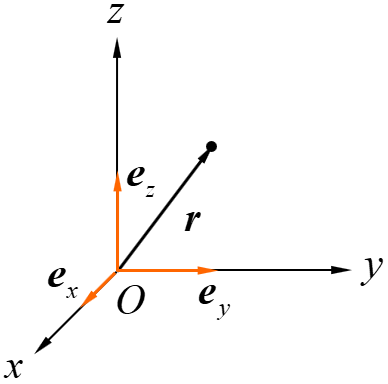
\includegraphics[width=1\textwidth]{figures/rectangular_coordinates.png}
			\caption{直角坐标系}\label{fig:rectangular_coordinates}
		\end{marginfigure}
	最典型的例子就是正交直角坐标系,或者说是Cartesian坐标系,如图\ref{fig:rectangular_coordinates}所示.在这种坐标系中,坐标线是直线,且彼此正交.通常,我们用$(x,y,z)$来表述直角坐标系中的点.
	\subsection{柱坐标系}
		\begin{marginfigure}
			\centering
			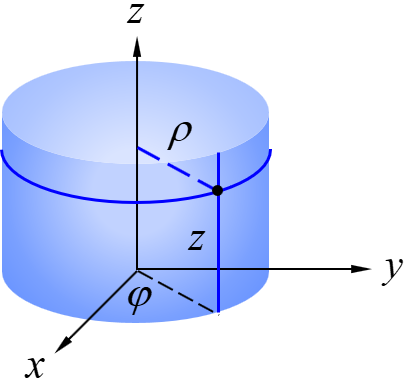
\includegraphics[width=1\textwidth]{figures/cylindrical_coordinates.png}
			\caption{柱坐标系}\label{fig:cylindrical_coordinates}
		\end{marginfigure}
		柱坐标系如图\ref{fig:cylindrical_coordinates}所示.通常,我们用$(r,\theta,z)$来表述柱坐标系中的点,其中线参数$r\in[0,+\infty)$,$z\in \mathbb{R}$,角参数$\theta\in[0,2\pi)$,这些参数构成的坐标线彼此正交.将一个由柱坐标参数描述的点变换到由直角坐标参数描述的点总是容易的,我们有它的坐标变换映射
		\begin{equation}\label{eq:rthetaz to xyz 1}
			(r,\theta,z)\mapsto(x,y,z),
		\end{equation}
		用坐标变换函数组表示就是
		\begin{equation}\label{eq:rthetaz to xyz 2}
			\begin{split}
				x(r,\theta,z)&=r\cos\theta;\\
				y(r,\theta,z)&=r\sin\theta;\\
				z(r,\theta,z)&=z.
			\end{split}
		\end{equation}
		我们注意到\ref{eq:rthetaz to xyz 2}是光滑的,通过计算可知其Jacobian$J=det(\partial(x,y,z)/\partial(r,\theta,z))$不为零,这意味着\ref{eq:rthetaz to xyz 2}还是可逆的.于是我们可以得到\ref{eq:rthetaz to xyz 1}的逆映射
		\begin{equation}\label{eq:xyz to rthetaz 1}
			(x,y,z)\mapsto(r,\theta,z),
		\end{equation}
		用坐标变换函数组表示就是
		\begin{equation}\label{eq:xyz to rthetaz 2}
			\begin{split}
				r(x,y,z)&=\sqrt{x^2+y^2};\\
				\theta(x,y,z)&=\arccos\left(\frac{x}{\sqrt{x^2+y^2}}\right);\\
				z(x,y,z)&=z.
			\end{split}
		\end{equation}
			
	\subsection{球坐标系}
			
		\begin{marginfigure}
			\centering
			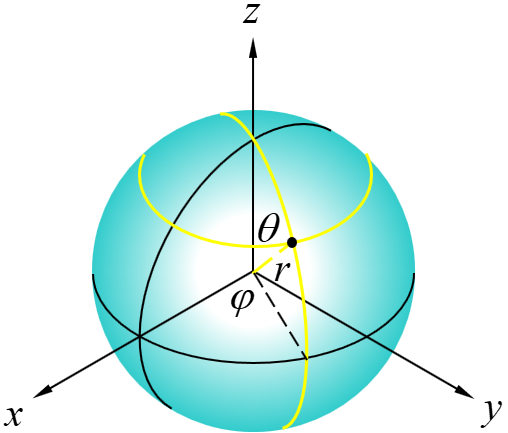
\includegraphics[width=1\textwidth]{figures/spherical_coordinates.png}
			\caption{球坐标系}\label{fig:spherical_coordinates}
		\end{marginfigure}
		球坐标系是除了直角坐标系以外最常用的坐标系,如图\ref{fig:spherical_coordinates}所示.我们用$(r,\theta,\varphi)$来描述球坐标系中的点,其中线参数$r\in[0,+\infty)$,角参数$\theta\in[0,\pi)$,$\varphi\in[0,2\pi)$,两个角参数通常隐含着系统的球对称性以及各向同性.与柱坐标系相同,球坐标系到直角坐标系也有坐标变换映射
		\begin{equation}\label{eq:rthetaphi to xyz 1}
			(r,\theta,\varphi)\mapsto(x,y,z),
		\end{equation}
		用坐标变换函数组表示就是
		\begin{equation}\label{eq:rthetaphi to xyz 2}
			\begin{split}
				x(r,\theta,\varphi)&=r\sin\theta \cos\varphi;\\
				y(r,\theta,\varphi)&=r\sin\theta \sin\varphi;\\
				z(r,\theta,\varphi)&=r\cos\theta.
			\end{split}
		\end{equation}
		同样的有直角坐标系到球坐标系的逆变换
		\begin{equation}\label{eq:xyz to rthetaphi 1}
			(r,\theta,\varphi)\mapsto(x,y,z),
		\end{equation}
		用坐标变换函数组表示就是
		\begin{equation}\label{eq:xyz to rthetaphi 2}
			\begin{split}
				r(x,y,z)&=\sqrt{x^2+y^2+z^2};\\
				\theta(x,y,z)&=\arccos\left(\frac{z}{\sqrt{x^2+y^2+z^2}}\right);\\
				\varphi(x,y,z)&=\arctan(\frac{y}{x}).
			\end{split}
		\end{equation}

		我还想再讲一讲超球坐标系,它是球坐标系进一步抽象的结果.$n$维的超球坐标系由$1$个线参数$x'^1\in[0,+\infty)$和$n-1$个角参数$x'^2,\cdots,x'^{n-2}\in[0,\pi)$,$x'^{n-1}\in[0,2\pi)$构成.超球坐标系到直角坐标系的坐标变换由如下映射给出
		\begin{equation}\label{eq:rthetaphi to xyz 3}
			\phi:R^n\rightarrow R^n;(x'^1,\cdots,x'^n)\mapsto(x^1,\cdots,x^n),
		\end{equation}
		用坐标变换函数组表示就是
		\begin{equation}\label{eq:rthetaphi to xyz 4}
			\begin{split}
				x^1(x'^1,\cdots,x'^n)&=x'^1\cos x'^2;\\
				x^2(x'^1,\cdots,x'^n)&=x'^1\sin x'^2\cos x'^3;\\
				x^3(x'^1,\cdots,x'^n)&=x'^1\sin x'^2\sin x'^3\cos x'^4;\\
				&\cdots\\
				x^{n-1}(x'^1,\cdots,x'^n)&=x'^1\sin x'^2\cdots \sin x'^{n-2}\cos x'^{n-1};\\
				x^{n}(x'^1,\cdots,x'^n)&=x'^1\sin x'^2\cdots \sin x'^{n-2}\sin x'^{n-1}.
			\end{split}
		\end{equation}
		如果我们令$n=3$,并进行参数变换$x^1=z$,$x^2=x$,$x^3=y$,以及$x'^1=r$,$x'^2=\theta$,$x'^3=\varphi$,则(\ref{eq:rthetaphi to xyz 4})就回到了(\ref{eq:rthetaphi to xyz 2})的情况.

		我们这就论述了三种常见的坐标系.这些坐标系都有一个特点,即坐标线相互垂直.通常我们也将这样的坐标系称为正交曲线坐标系.当然,还有其他的正交曲线坐标系,例如圆环坐标系、椭球坐标系,等等,我们不再一一列举.但你可能会问:“有没有坐标线相互不正交的曲线坐标系?”那么我的回答是:“当然有.”实际上,坐标线相互不正交的坐标系才是一般情况.为了描述一般情况下的坐标系,我们将坐标变换函数组统一的记成$x^\mu(x'^\nu)$的形式,其中$\mu$指标表示“取坐标变换函数组中的第$\mu$个函数$x^\mu$”,$\nu$指标表示“取定函数$x^\mu$后,取函数的第$\nu$个参数”.这样的表述方法称为\textbf{抽象指标}记号,抽象指标在取定数值后成为\textbf{具体指标}.后面我们会看到,这样的表述方法是非常方便的.